\section{Theory}

\subsection{Introduction}

A \emph{tree} is an abstract hierarchical data type that connects \emph{nodes}
via \emph{edges}. Each node in a tree is connected to a single \emph{parent
node} with the exception of the \emph{root node}, which has no parent.
Additionally, each node may be connected to multiple \emph{child nodes}.
In DGTile, we use a \emph{binary tree}, a \emph{quadtree}, and an \emph{octree}
to enable mesh adaptivity in one, two, and three spatial dimensions,
respectively. In a binary tree, quadtree, and octree each \emph{internal node}
is connected to exactly two, four, and eight \emph{child nodes}. In contrast,
a \emph{leaf node} is any node in the tree that contains no children. The
\emph{level} of a node in the tree is its distance away from the rood node,
where the \emph{distance} is the number of edges along the shortes path
between two nodes. The root node in a tree has a level of $0$.

\subsection{Uniquely Identifying Nodes in the Tree}

\documentclass[border={20pt 20pt 20pt 20pt},preview]{standalone}
\usepackage{pgfplots}
\usepackage{subcaption}
\usepackage{amsmath}
\usepackage{amssymb}
\pgfplotsset{compat=1.16}
\usepackage{tikz}

\begin{document}

\begin{figure}[ht!]
\begin{subfigure}{0.33\textwidth}
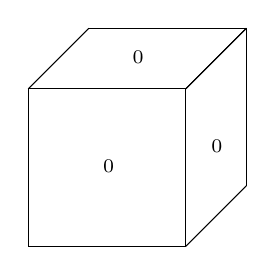
\begin{tikzpicture}[scale=0.5]
\foreach \x in{0,4}
{   \draw (0,\x ,4) -- (4,\x ,4);
    \draw (\x ,0,4) -- (\x ,4,4);
    \draw (4,\x ,4) -- (4,\x ,0);
    \draw (\x ,4,4) -- (\x ,4,0);
    \draw (4,0,\x ) -- (4,4,\x );
    \draw (0,4,\x ) -- (4,4,\x );
}
\node at (0.5,0.5) {\scriptsize $0$};
\node at (3.25,1.0) {\scriptsize $0$};
\node at (1.25,3.25) {\scriptsize $0$};
\end{tikzpicture}
\caption{Level 0}
\end{subfigure}%
\begin{subfigure}{0.33\textwidth}
\centering
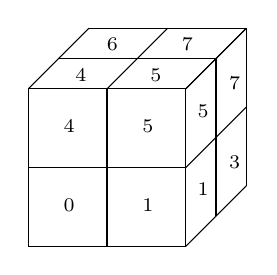
\begin{tikzpicture}[scale=0.5]
\foreach \x in{0,2,4}
{   \draw (0,\x ,4) -- (4,\x ,4);
    \draw (\x ,0,4) -- (\x ,4,4);
    \draw (4,\x ,4) -- (4,\x ,0);
    \draw (\x ,4,4) -- (\x ,4,0);
    \draw (4,0,\x ) -- (4,4,\x );
    \draw (0,4,\x ) -- (4,4,\x );
}
\node at (-0.5,-0.5) {\scriptsize $0$};
\node at (1.5,-0.5) {\scriptsize $1$};
\node at (-0.5,1.5) {\scriptsize $4$};
\node at (1.5,1.5) {\scriptsize $5$};
\node at (2.9,-0.1) {\scriptsize $1$};
\node at (3.7, 0.6) {\scriptsize $3$};
\node at (2.9, 1.9) {\scriptsize $5$};
\node at (3.7, 2.6) {\scriptsize $7$};
\node at (-0.2, 2.8) { \scriptsize $4$};
\node at (1.7, 2.8) { \scriptsize $5$};
\node at (0.6, 3.6) { \scriptsize $6$};
\node at (2.5, 3.6) { \scriptsize $7$};
\end{tikzpicture}
\caption{Level 1}
\end{subfigure}%
\begin{subfigure}{0.33\textwidth}
\centering
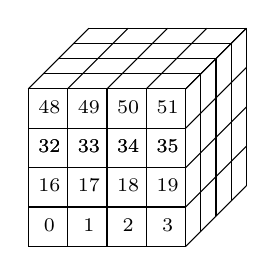
\begin{tikzpicture}[scale=0.5]
\foreach \x in{0,...,4}
{   \draw (0,\x ,4) -- (4,\x ,4);
    \draw (\x ,0,4) -- (\x ,4,4);
    \draw (4,\x ,4) -- (4,\x ,0);
    \draw (\x ,4,4) -- (\x ,4,0);
    \draw (4,0,\x ) -- (4,4,\x );
    \draw (0,4,\x ) -- (4,4,\x );
}
\node at (-1.0,-1.0) {\scriptsize $0$};
\node at ( 0.0,-1.0) {\scriptsize $1$};
\node at ( 1.0,-1.0) {\scriptsize $2$};
\node at ( 2.0,-1.0) {\scriptsize $3$};
\node at (-1.0, 0.0) {\scriptsize $16$};
\node at ( 0.0, 0.0) {\scriptsize $17$};
\node at ( 1.0, 0.0) {\scriptsize $18$};
\node at ( 2.0, 0.0) {\scriptsize $19$};
\node at (-1.0, 1.0) {\scriptsize $32$};
\node at ( 0.0, 1.0) {\scriptsize $33$};
\node at ( 1.0, 1.0) {\scriptsize $34$};
\node at ( 2.0, 1.0) {\scriptsize $35$};
\node at (-1.0, 1.0) {\scriptsize $32$};
\node at ( 0.0, 1.0) {\scriptsize $33$};
\node at ( 1.0, 1.0) {\scriptsize $34$};
\node at ( 2.0, 1.0) {\scriptsize $35$};
\node at (-1.0, 2.0) {\scriptsize $48$};
\node at ( 0.0, 2.0) {\scriptsize $49$};
\node at ( 1.0, 2.0) {\scriptsize $50$};
\node at ( 2.0, 2.0) {\scriptsize $51$};
\end{tikzpicture}
\caption{Level 2}
\end{subfigure}
\caption*{Local level-specific identifiers: $\text{id}(l,i,j,k)$ for an octree.}
\label{fig:tree_level_ids}
\end{figure}

\end{document}


For the purposes of identifying, storing, modifying, and computing adjacencies
of leaves in the tree, it is useful to assign unique identifiers to every
possible node in the tree at every possible level. These identifiers are
computed using simple integer arithmetic. At every potential level $l$ in the
octree, we can assign a level-specific identifier $\id(l,i,j,k)$ to a
potential node in the tree given the node's $ijk$ Cartesian grid location
at that level. Presently, we consider the following choice for the
level-specific identifier
%
\begin{equation}
\id(l,i,j,k) = i + 2^l(j + k 2^l)
\end{equation}
%
where identifiers are strided the quickest along the $x$-axis and slowest
along the $z$-axis. Note that for a two-dimensional tree $k$ will always
be $0$ and likewise, for a one-dimensional tree $k$ and $j$ will always
be $0$. Figure~\ref{fig:tree_level_ids} illustrates level-specific identifiers
for levels $l=0,1,2$ for an octree, where the $x$-axis extends from the left to
right of the page, the $y$-axis extends from out to into the page, and the
$z$-axis extends from bottom to top of the page. This convention will be used
in subsequent figures as well. For compatability with \texttt{C++}, all indices
start from $0$.

\begin{figure}[ht!]
\begin{subfigure}{0.33\textwidth}
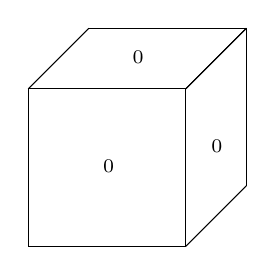
\begin{tikzpicture}[scale=0.5]
\foreach \x in{0,4}
{   \draw (0,\x ,4) -- (4,\x ,4);
    \draw (\x ,0,4) -- (\x ,4,4);
    \draw (4,\x ,4) -- (4,\x ,0);
    \draw (\x ,4,4) -- (\x ,4,0);
    \draw (4,0,\x ) -- (4,4,\x );
    \draw (0,4,\x ) -- (4,4,\x );
}
\node at (0.5,0.5) {\scriptsize $0$};
\node at (3.25,1.0) {\scriptsize $0$};
\node at (1.25,3.25) {\scriptsize $0$};
\end{tikzpicture}
\caption{Level 0}
\end{subfigure}%
\begin{subfigure}{0.33\textwidth}
\centering
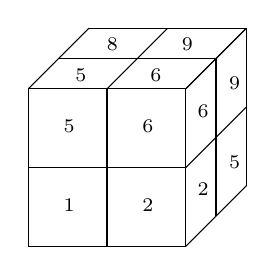
\begin{tikzpicture}[scale=0.5]
\foreach \x in{0,2,4}
{   \draw (0,\x ,4) -- (4,\x ,4);
    \draw (\x ,0,4) -- (\x ,4,4);
    \draw (4,\x ,4) -- (4,\x ,0);
    \draw (\x ,4,4) -- (\x ,4,0);
    \draw (4,0,\x ) -- (4,4,\x );
    \draw (0,4,\x ) -- (4,4,\x );
}
\node at (-0.5,-0.5) {\scriptsize $1$};
\node at (1.5,-0.5) {\scriptsize $2$};
\node at (-0.5,1.5) {\scriptsize $5$};
\node at (1.5,1.5) {\scriptsize $6$};
\node at (2.9,-0.1) {\scriptsize $2$};
\node at (3.7, 0.6) {\scriptsize $5$};
\node at (2.9, 1.9) {\scriptsize $6$};
\node at (3.7, 2.6) {\scriptsize $9$};
\node at (-0.2, 2.8) { \scriptsize $5$};
\node at (1.7, 2.8) { \scriptsize $6$};
\node at (0.6, 3.6) { \scriptsize $8$};
\node at (2.5, 3.6) { \scriptsize $9$};
\end{tikzpicture}
\caption{Level 1}
\end{subfigure}%
\begin{subfigure}{0.33\textwidth}
\centering
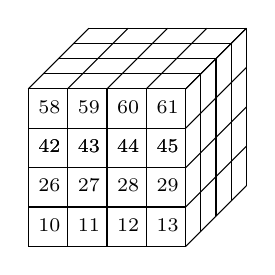
\begin{tikzpicture}[scale=0.5]
\foreach \x in{0,...,4}
{   \draw (0,\x ,4) -- (4,\x ,4);
    \draw (\x ,0,4) -- (\x ,4,4);
    \draw (4,\x ,4) -- (4,\x ,0);
    \draw (\x ,4,4) -- (\x ,4,0);
    \draw (4,0,\x ) -- (4,4,\x );
    \draw (0,4,\x ) -- (4,4,\x );
}
\node at (-1.0,-1.0) {\scriptsize $10$};
\node at ( 0.0,-1.0) {\scriptsize $11$};
\node at ( 1.0,-1.0) {\scriptsize $12$};
\node at ( 2.0,-1.0) {\scriptsize $13$};
\node at (-1.0, 0.0) {\scriptsize $26$};
\node at ( 0.0, 0.0) {\scriptsize $27$};
\node at ( 1.0, 0.0) {\scriptsize $28$};
\node at ( 2.0, 0.0) {\scriptsize $29$};
\node at (-1.0, 1.0) {\scriptsize $42$};
\node at ( 0.0, 1.0) {\scriptsize $43$};
\node at ( 1.0, 1.0) {\scriptsize $44$};
\node at ( 2.0, 1.0) {\scriptsize $45$};
\node at (-1.0, 1.0) {\scriptsize $42$};
\node at ( 0.0, 1.0) {\scriptsize $43$};
\node at ( 1.0, 1.0) {\scriptsize $44$};
\node at ( 2.0, 1.0) {\scriptsize $45$};
\node at (-1.0, 2.0) {\scriptsize $58$};
\node at ( 0.0, 2.0) {\scriptsize $59$};
\node at ( 1.0, 2.0) {\scriptsize $60$};
\node at ( 2.0, 2.0) {\scriptsize $61$};
\end{tikzpicture}
\caption{Level 2}
\end{subfigure}
\caption{Global unique identifiers: $\ID(l,i,j,k)$ for an octree}
\label{fig:tree_global_IDs}
\end{figure}


A unique identifier for each node can then be found by computing a
level-specific offset $\delta(d,l)$ that denotes the total number of potential
nodes in the tree up to the current level $l$. Here $d=1,2,3$ denotes the
spatial dimension of the mesh. This offset is computed as
%
\begin{equation}
\delta(d,l) = \sum_{n=0}^l (2^d)^n = \frac{(2^d)^l - 1}{2^d - 1}
\end{equation}
%
and the resultant unique node identifier in the octree is specified as the
sum of the offset $\delta(d,l)$ and the level-specific identifier
$\id(l,i,j,k)$:
%
\begin{equation}
\ID(d,l,i,j,k) = \delta(d,l) + \id(l,i,j,k)
\end{equation}
%
Figure~\ref{fig:tree_global_IDs} illustrates unique identifiers $\ID$ for
levels $l=0,1,2$ for an octree.

\subsection{Octree Representation}

\subsection{Z-curve Ordering}

\subsection{Leaf Adjacencies}

\subsection{Modifying the Tree}

\subsection{Ensuring Balanced Leaf Interfaces}
